\documentclass[]{article}

\usepackage{amsmath}
\usepackage{graphicx}

%opening
\title{Optimizing variance decomposition}
\author{Raphael Scherrer}

\begin{document}

\maketitle

Phenotypic variance can be decomposed into genetic and environmental variance, the former of which can be decomposed into additive and non-additive variance, where non-additive variance includes dominance and epistatic variance. One way of calculating each of these variance components, for a given locus, involves looping a first time through individuals to compute the additive and dominance expectations, then looping again to record the deviations of each individual to these expectations, which can be attributed to epistasis (if environmental variance is negligible). Here, we derive the decomposed locus-specific phenotypic variance in terms of sums and sums of squared locus-specific genetic values across the population, allowing to loop only once through the population of individuals and therefore increase the efficiency of our algorithm. The equations derived here are used and compared to regular variance calculation in the accompanying R script.\\

In our simulation model, the phenotype of an individual is an accumulation of locus-specific genetic effects (which themselves incorporate independent and interaction effects, see Methods). Because we know these locus-specific genetic values, i.e. the contribution of each locus, we decompose their variance into its additive and non-additive components, with estimates for each single locus. Note that in empirical systems, the genetic value of each locus is typically unknown and estimates of the additive and non-additive effects attributable to each locus are done by finding effects on the phenotype of the whole individual, which may also be under environmental effects, thus complexifying the matter. Here, we are interested in these variance estimates as diagnostic tools to help us understand the dynamics unfolding in our simulations at the genomic level, not in deriving variance estimates similar to what would be available to the empiricist. We therefore focus our locus-specific variance decomposition on explaining the variance in locus-specific genetic values instead of whole individual phenotypic values. Note that because of this, we also do not need to take into account environmental effects, which are added to the individual's phenotype after the genetic effect of its whole genome has been computed.\\

We use a classical linear regression to decompose the variance in genetic values, which is also the phenotypic variance when there are no environmental effects, into additive and non-additive components (Figure \ref{fig:regression}). We then compute quantitative genetics F-statistics analogous to the $F_{ST}$ statistic to assess the partitioning of these variance components between the two incipient species in our model of speciation, to provide us with more insights into the mechanisms through which the genome evolves towards speciation.\\

The linear regression is done as follows. Suppose that a population of $N$ individuals is genetically diverse for a given diploid locus $i$, which underlies variation in a particular encoded trait of interest. Each individual $k$ is characterized by its allele count $q_{ijk}$, or genotype $j$, which in a diploid species can take the values 0, 1 or 2; and its genetic value at that locus $g_{ijk}$, i.e. the contribution of that locus to that individual's trait value. The genetic values $g_i$ are regressed against their respective allele counts $q_i$ across the whole population. The regression line represents the additive expectation, i.e. the genetic value expected under additivity, and its slope is the average mutational effect at locus $i$, $\alpha_i$. The breeding value $\beta_{ij}$ of each genotype $j$ is the deviation between the additive expectation of this genotype, $g^*_{ij}$, and the mean genetic value of the population, $\bar{g}_i$. The additive variance $V_{A,i}$ is the variance in breeding values across the population, that is,

\begin{align} 
V_{A,i} &= E(\beta_{ij}^2) - E(\beta_{ij})^2\\
&= \sum_j p_{ij} \, \beta_{ij}^2 - \bigg( \sum_j p_{ij} \, \beta_{ij} \bigg)^2
\end{align}

where $p_{ij}$ is the proportion of the frequency of genotype $j$ at locus $i$.\\

The deviation in genetic value from the additive expectation due to dominance for genotype $j$, $\delta_{ij}$, is the difference between the mean genetic value within genotype $j$, $\tilde{g}_{ij}$, and its additive expectation $g^*_{ij}$. The genetic variance attributable to dominance is calculated as the variance in $\delta_{ij}$, that is,

\begin{align}
V_{D,i} &= E(\delta_{ij}^2) - E(\delta_{ij})^2\\
&= \sum_j p_{ij} \, \delta_{ij}^2 - \bigg( \sum_j p_{ij} \, \delta_{ij} \bigg)^2
\end{align}

The residual variance, after accounting for the additive effects and genotype-specific dominance effects, is attributed to the genetic background, i.e. epistasis (again, there are no environmental effects at the locus level). Residuals $\epsilon_{ijk}$ are, for each individual $k$ within genotype $j$, the deviations between the individual's genetic value $g_{ijk}$ and the mean genetic value of its genotype-group, $\tilde{g}_{ij}$. The epistatic variance is therefore given by

\begin{align} 
V_{I,i} &= E(\epsilon_{ijk}^2) - E(\epsilon_{ijk})^2\\
&= \frac{1}{N} \sum_k \epsilon_{ijk}^2 - \bigg( \frac{1}{N} \sum_k \epsilon_{ijk} \bigg)^2
\end{align}

Because $\epsilon_{ijk} = g_{ijk} - \tilde{g}_{ij}$ and $\epsilon_{ijk}^2 = g_{ijk}^2 - 2 \, \tilde{g}_{ij} \, g_{ijk} + \tilde{g}_{ij}^2$, 

\begin{equation}
\sum_k \epsilon_{ijk} = \sum_k g_{ijk} - \sum_j n_{ij} \, \tilde{g}_{ij}
\end{equation}

and

\begin{equation}
\sum_k \epsilon_{ijk}^2 = \sum_k g_{ijk}^2 - 2 \, \sum_k \tilde{g}_{ij} \, g_{ijk} + \sum_j n_{ij} \, \tilde{g}_{ij}^2
\end{equation}

where 

\begin{equation}
\sum_k \tilde{g}_{ij} \, g_{ijk} = \sum_j \tilde{g}_{ij} \, \sum_{k_j} g_{ijk_j}
\end{equation}

where $k_j$ denotes an individual belonging to genotype $j$.\\

We can derive the non-additive variance in a similar way, as the variance in deviations from the regression line, that is, in deviations $\gamma_{ijk}$ due to both dominance and epistasis, equal to $g_{ijk} - g^*_{ij}$. The equation for the non-additive variance $V_{N,i}$ is therefore the same as for the interaction variance $V_{I,i}$, except that $\tilde{g}_{ij}$ is replaced with $g^*_{ij}$ (so we do not rewrite it here for brevity).\\

Note that the various variance components include expectations of residual deviations (such as $E(\beta_{ij})$ or $E(\gamma_{ijk})$) to a linear expectation. These expectations are zero when calculating variances across the whole population. However, to calculate the proportion of the variance attributable to each ecotype (i.e. incipient species), we must calculate the variance in the said residual deviations \textit{within} each ecotype and compare it to the population-wide variance, and the within-ecotype distribution of residuals needs not be centered on zero.\\

The aforementioned equations suggest that all locus-specific variance components can be derived from three 3-by-4 matrices, with one row per ecotype plus a third row for the whole population, and one column per genotype plus a fourth column for the whole population. The first matrix records the number of individuals in each category (the value in the third row, fourth column is $N$). The second matrix records the sums of genetic values in each category. The third matrix records the sums of squared genetic values in each category. These matrices can be computed by looping a single time through the population for a given locus. Once the matrices are available, the slope $\alpha_i$ of the linear regression can be computed as the ratio between the covariance of $g_i$ and $q_i$, and the variance in $q_i$ across the population. The breeding values $\beta_{ij}$ can then be computed for each genotype $j$ as $\alpha_i \, (q_{ij} - \bar{q_i})$. The genotype-means $\tilde{g}_{ij}$ can then be compared to the additive expectations $g^*_{ij}$ to find the dominance deviations $\delta_{ij}$. The individual-specific residuals, i.e. $\epsilon_{ijk}$ and $\gamma_{ijk}$ can be found using the sums and sums of squares already computed, without having to loop again through the population and record their deviations from additive and dominance expectations.

\begin{figure}
	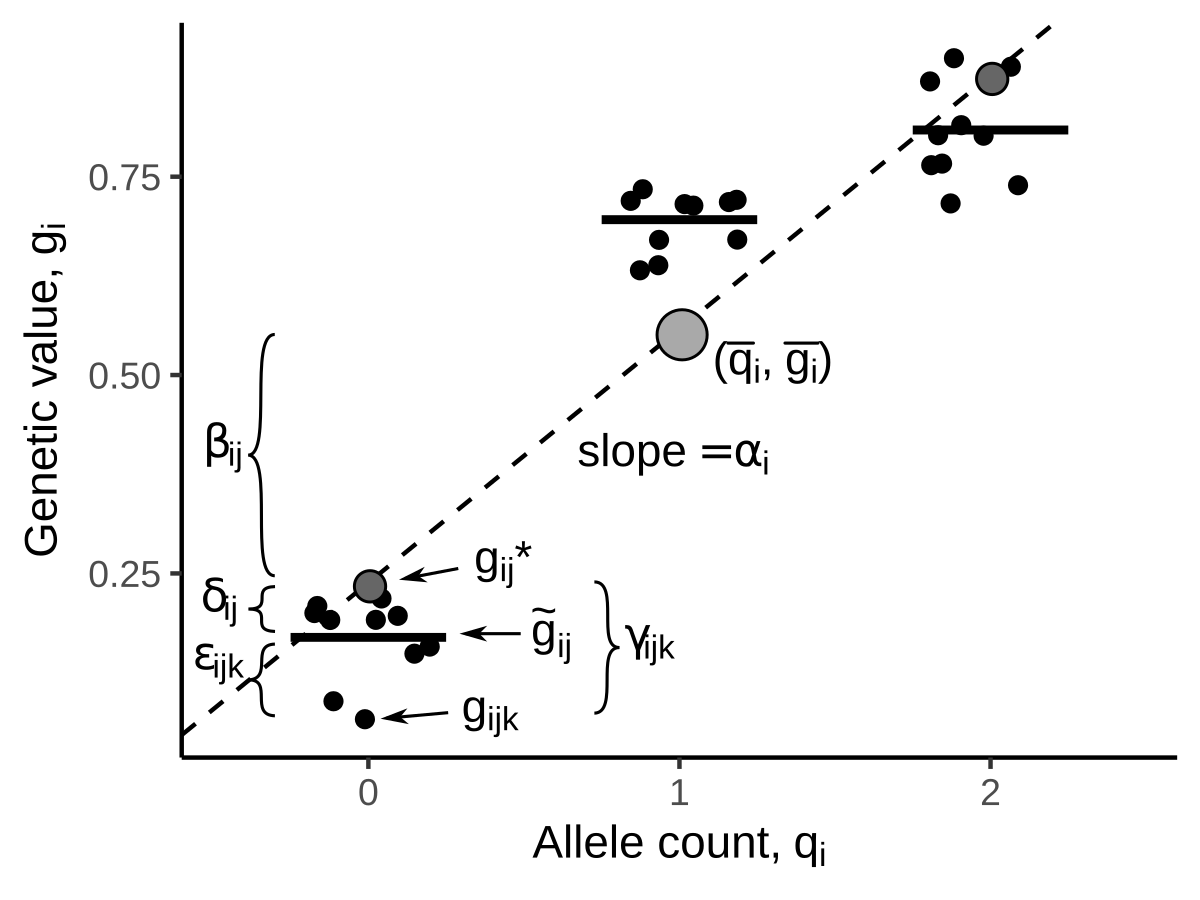
\includegraphics{variance-decomp-custom.png}
	\caption{Schematic representation of the a locus-specific variance decomposition procedure. For a given locus $i$, the genetic value $g$ is regressed against the allele count $q$ across all individuals in the population. Deviations of genotype-means (horizontal bars) to the regression line are attributed to dominance, while residuals are attributed to epistatic interactions.}
	\label{fig:regression}
\end{figure}


\end{document}
